\documentclass[uct_visualisation_thesis.tex]{subfiles}

\section{Wymagania do instalacji}
\begin{enumerate}
	\item Około 150 MB wolnego miejsca przestrzeni dyskowej,
	\item Karta graficzna.
\end{enumerate}
\section{Instrukcja instalacji Windows}
Aby zainstalować aplikację na lokalnym dysku należy uruchomić plik instalacyjny \textbf{UCTVisualisationSetup.exe}. Następnie ukaże się okno przeprowadzające użytkownika przez proces instalacji. Należy wybrać folder docelowy i kliknąć na przycisk \textit{Install}. Po zakończeniu procesu można zamknąć okno instalacji zaznaczając przedtem \textit{Run UCT Visualisation}, aby bezpośrednio po zamknięciu instalatora uruchomiła się aplikacja.\\
Zainstalowana aplikacja znajduje się w folderze wskazanym przez użytkownika podczas instalacji w katalogu \textbf{UCT Visualisation}. Aby uruchomić aplikację należy w niego wejść i uruchomić plik \textbf{UCT Visualisation.exe}.
Okno instalacji powinno przypominać to, ukazane na rysunku \ref{rys:instalacja}.

\begin{figure}[h!]
	\centering
	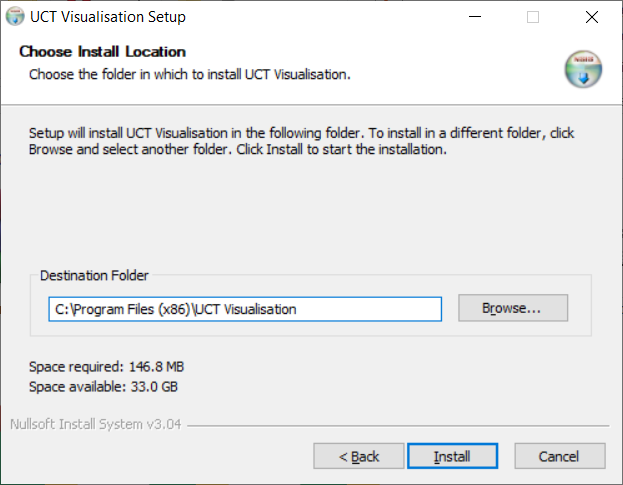
\includegraphics[width=0.7\textwidth]{instalacja}
	\caption{Okno instalacji programu}
	\label{rys:instalacja}
\end{figure}

\section{Instrukcja instalacji Linux}
\section{Instrukcja użytkownika}
